\subsection{Configure slave GBTx to use master SCA channel}
This setup is required to program a slave via a master SCA channel.
In a typical scenario, the master is connected to a MiniDAQ so that programming
the slave using the MiniDAQ directly\footnote{
    MiniDAQ $\to$ master GBTx $\to$ slave GBTx.
}is possible.
Follow \autoref{fig:master-sca} to connect a slave GBTx to the SCA channel of a
master GBTx board.

\begin{center}
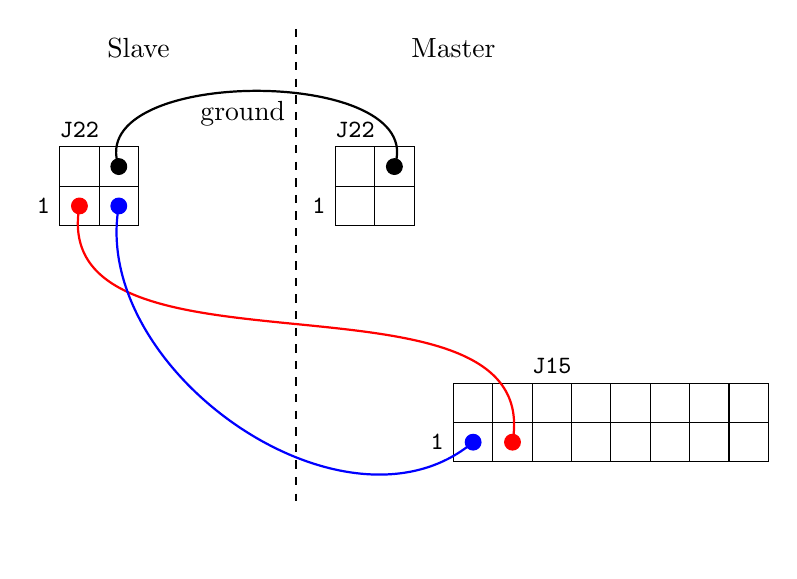
\begin{tikzpicture}
    % Separation
    \draw [thick,dashed] (0,3) to (0,-3);
    \coordinate (Slave) at (-2,3);
    \coordinate (Master) at (2,3);
    \node at (Slave) [below] {Slave};
    \node at (Master) [below] {Master};

    % Pins & labels on the slave
    \draw (-3,1) rectangle (-2.5,1.5);
    \draw (-2.5,1) rectangle (-2,1.5);
    \draw (-3,0.5) rectangle (-2.5,1);
    \draw (-2.5,0.5) rectangle (-2,1);
    \coordinate (A) at (-2.75,1.5);
    \node at (A) [above] {\small\texttt{J22}};
    \coordinate (B) at (-3,0.75);
    \node at (B) [left] {\small\texttt{1}};

    % Pins & labels on the master
    \draw (0.5,1) rectangle (1,1.5);
    \draw (1,1) rectangle (1.5,1.5);
    \draw (0.5,0.5) rectangle (1,1);
    \draw (1,0.5) rectangle (1.5,1);
    \coordinate (C) at (0.75,1.5);
    \node at (C) [above] {\small\texttt{J22}};
    \coordinate (D) at (0.5,0.75);
    \node at (D) [left] {\small\texttt{1}};
    % Another pin
    \draw (2,-1.5) rectangle (6,-2.5);
    \draw (2,-2) to (6,-2);
    \draw (2.5,-1.5) to (2.5,-2.5);
    \draw (3,-1.5) to (3,-2.5);
    \draw (3.5,-1.5) to (3.5,-2.5);
    \draw (4,-1.5) to (4,-2.5);
    \draw (4.5,-1.5) to (4.5,-2.5);
    \draw (5,-1.5) to (5,-2.5);
    \draw (5.5,-1.5) to (5.5,-2.5);
    \coordinate (E) at (3.25,-1.5);
    \node at (E) [above] {\small\texttt{J15}};
    \coordinate (F) at (2,-2.25);
    \node at (F) [left] {\small\texttt{1}};

    % Single grounding cable
    \draw [black,fill] (-2.25,1.25) circle [radius=0.1];
    \draw [black,fill] (1.25,1.25) circle [radius=0.1];
    \draw [thick,out=110,in=70] (-2.25,1.25)
    to node [below,xshift=-0.5em] {ground} (1.25,1.25);

    % 2x1 cross connector
    \draw [red,fill] (-2.75,0.75) circle [radius=0.1];
    \draw [red,fill] (2.75,-2.25) circle [radius=0.1];
    \draw [thick,red,out=-100,in=80] (-2.75,0.75) to (2.75,-2.25);
    \draw [blue,fill] (-2.25,0.75) circle [radius=0.1];
    \draw [blue,fill] (2.25,-2.25) circle [radius=0.1];
    \draw [thick,blue,out=-100,in=220] (-2.25,0.75) to (2.25,-2.25);
\end{tikzpicture}
\captionof{figure}{Schematic for slave to master SCA setup.}
\label{fig:master-sca}
\end{center}

\begin{leftbar}
    The black ground cable can be connected to any of the ground pin on the
    master GBTx.
\end{leftbar}

\begin{leftbar}
    There is a 2x1 to 2x1 cross-type cable made in-house to replace the
    red-blue cables.
    To use that cable, make sure the two 2x1 connectors have the same
    orientation (e.g.\ the sides \emph{without} metal contact are both facing
    up).
\end{leftbar}
